\chapter{Discussion}\label{ch:Discussion}


\section{GUI}
When a user of the system lay their eyes on the GUI, the first elements, they will see, are inputs for how many columns and rows should be in the grid that makes up the system as can be seen in \autoref{fig:GUI_screenshot_1}. Even though the user might be quite knowledgeable about networking, the will only be able to guess what this grid is. Therefore, an easy to implement solution could be to provide a simple description of the use case of the system. An even better solution could be to provide an image that changed along with the users input, and then provide some visualisation of the size of the grid such as axes to clarify even further that the user is changing the graph or grid that will make up the area where the devices in the network simulation can occupy.

\begin{figure}[H]
  \centering
  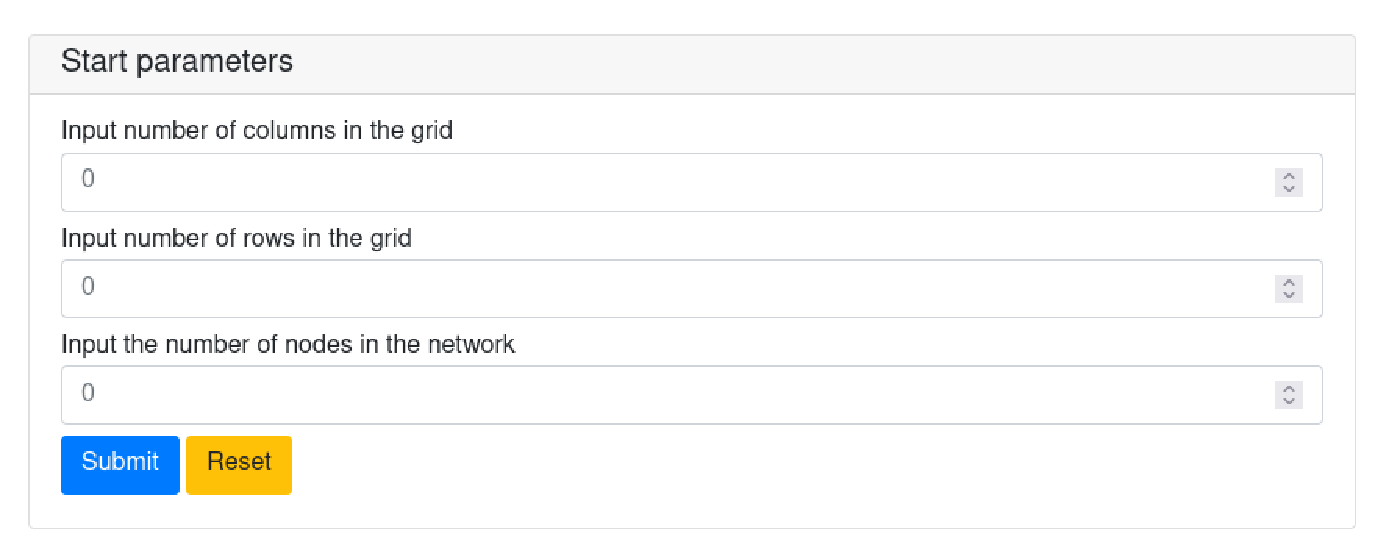
\includegraphics[width=\textwidth]{GUI_screenshot_1.pdf}
  \caption{A screenshot of the first elements that are displayed when a user opens the GUI.}
  \label{fig:GUI_screenshot_1}
\end{figure}

Then, after the 


\section{Network}
As has already been described in \autoref{sec:Class_diagram_Network} and in the rest of \autoref{sec:Class_diagram}, a better implementation of how the system currently is implemented would have tried to get as close to functional cohesion as possible in order clarify and improve which object does what. As the implementation currently is, a name that more precisely describes the functionality of the \code{simulation} object would be \code{simulation\_and\_networking}. Of course, it must be acknowledged that complete functional cohesion will not make sense in this project, where 


\section{Device}


\subsection{Node}


\subsection{Gateway}


\section{Simulation}



































